\section{Appendix A}
\label{AppendixA}
\subsection{Sample point/lines used in Comsol}

Data is gathered at specific locations in the battery models.
For the 6S1P, the middle point is blabla
\begin{figure} [H]
	\centering
	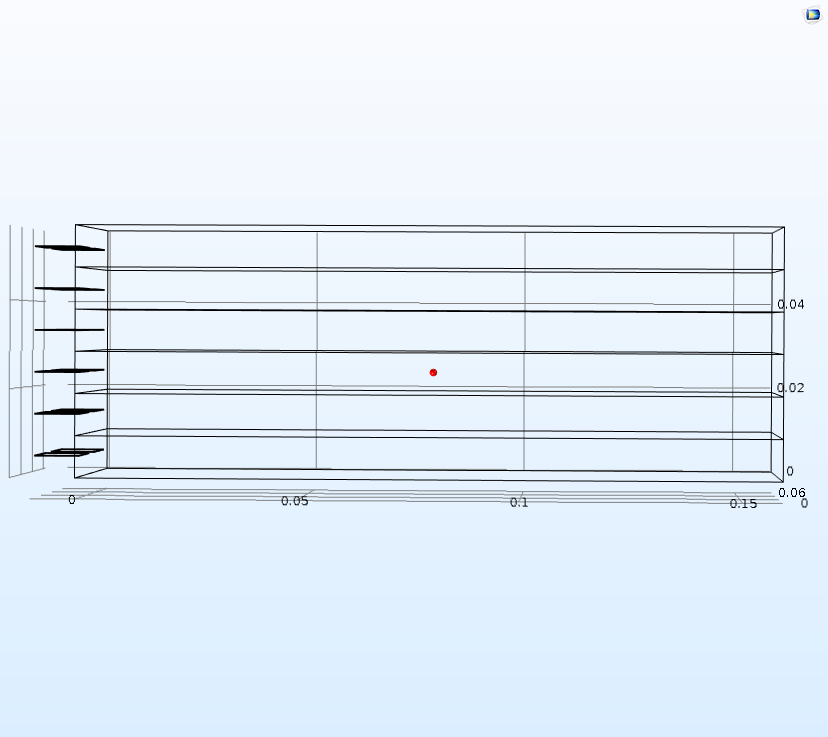
\includegraphics[width=0.5\linewidth]{Figures/6_Point_in_3D.png}
	\caption{Point of measurement in 6S1P simulation.}
   \label{Fig:6_1}
\end{figure}
\begin{figure} [H]
	\centering
	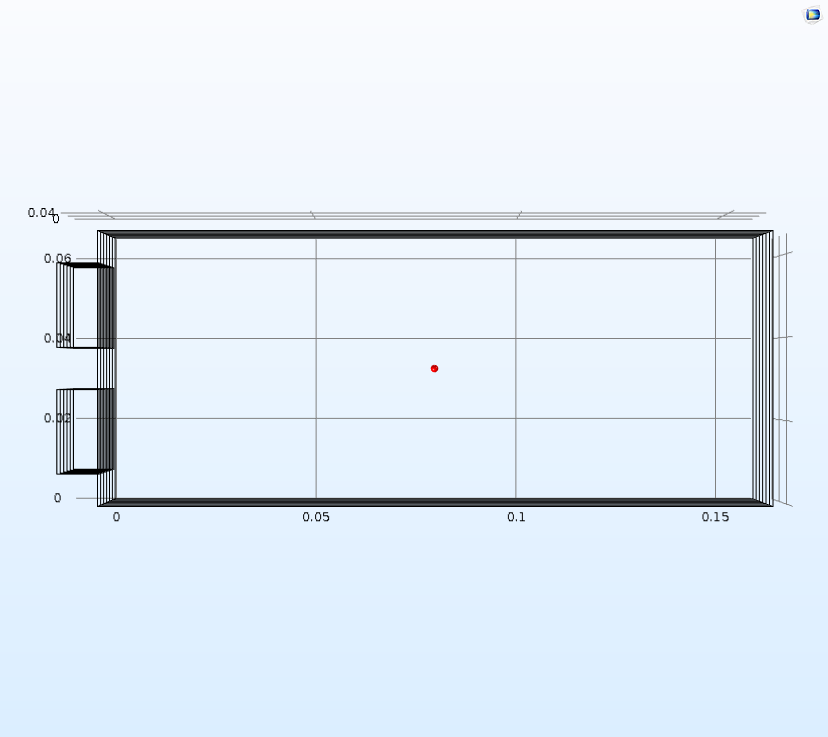
\includegraphics[width=0.5\linewidth]{Figures/6_Point_in_3D_2.png}
	\caption{Point of measurement in 6S1P simulation.}
   \label{Fig:6_2}
\end{figure}

\begin{figure} [H]
	\centering
	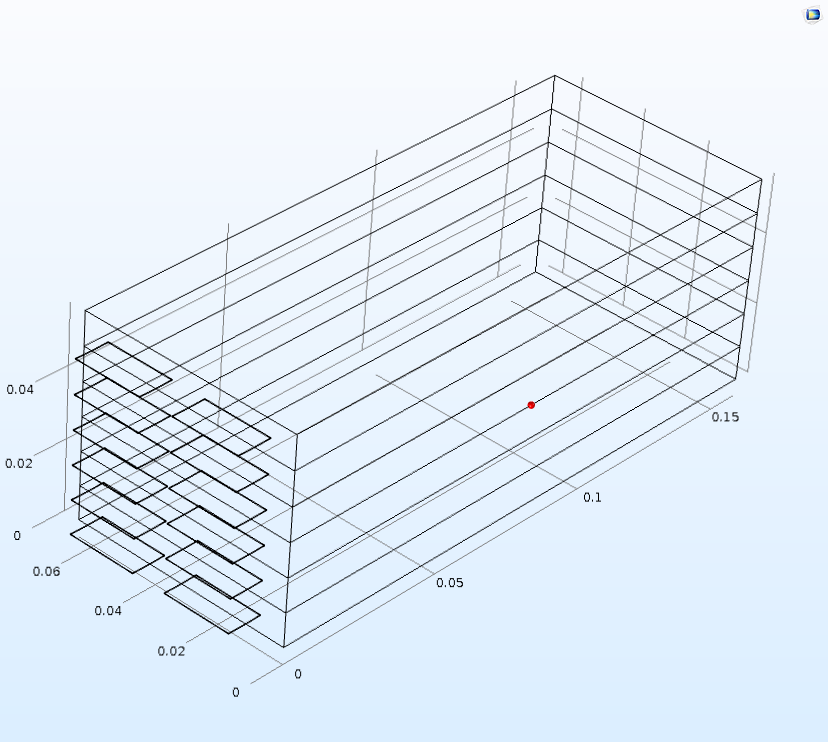
\includegraphics[width=0.5\linewidth]{Figures/6_Point_in_3D_3.png}
	\caption{Point of measurement in 6S1P simulation.}
   \label{Fig:6_3}
\end{figure}

\begin{figure} [H]
	\centering
	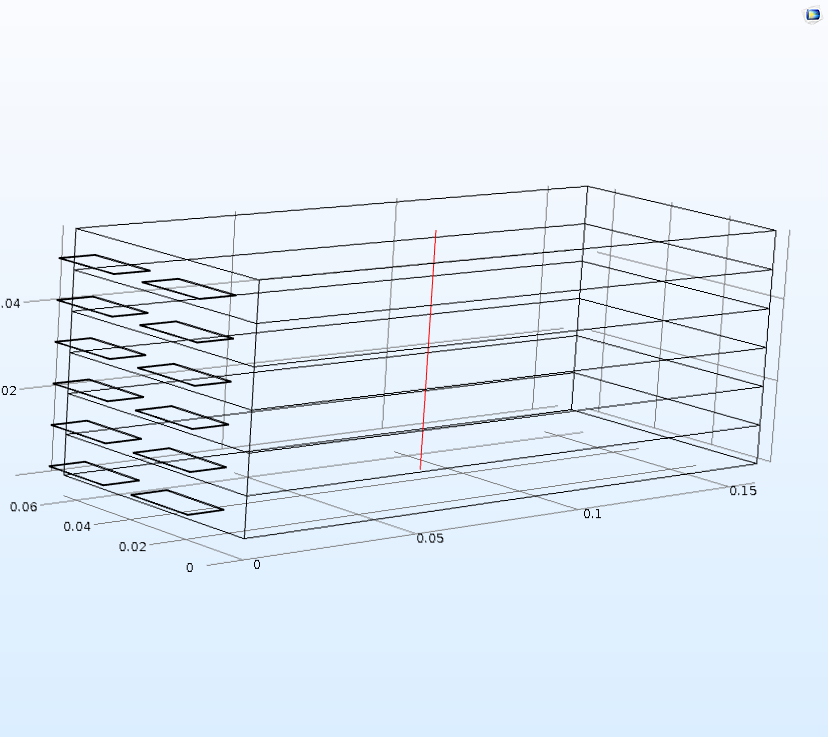
\includegraphics[width=0.5\linewidth]{Figures/LineOutPlane.png}
	\caption{Point of measurement in 6S1P simulation.}
   \label{Fig:6_4}
\end{figure}

\begin{figure} [H]
	\centering
	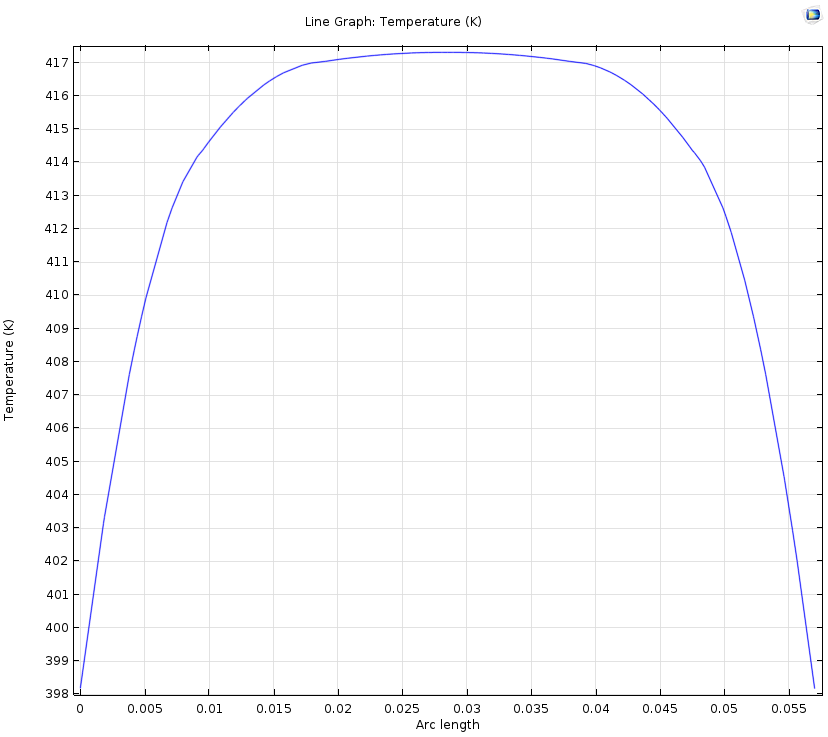
\includegraphics[width=0.5\linewidth]{Figures/300s_10h_180A_2mOhm_OutOfPlaneLast_NoPouch.png}
	\caption{Point of measurement in 6S1P simulation.}
   \label{Fig:6_5}
\end{figure}



\newpage
